\documentclass[%
aip,
amsmath,amssymb,
preprint,%
%reprint,%
%author-year,%
%author-numerical,%
]{revtex4-2}

\usepackage{hyperref}

\usepackage{siunitx}
\DeclareSIUnit\rydberg{Ry}
\usepackage{tikz}
\usepackage{paralist}
\usepackage[version=4]{mhchem}
\usepackage{rotating}
\usepackage{chngcntr}


\def\dbe{\ensuremath{\Delta\text{BE}}}

\renewcommand{\thetable}{S\arabic{table}}
\renewcommand{\thefigure}{S\arabic{figure}}

\NewDocumentCommand{\cpx}{O{}m}{SJ\IfNoValueTF{#1}{}{\textsuperscript{#1}}+$E_{ref} = #2$}

\renewcommand{\thepage}{S\arabic{page}}

\begin{document}
	\title{Prediction of XPS binding energies for molecules grafted on calcium surfaces\\ Supplementary materials}
	
	\author{Pierre Beaujean}
	\email{pierre.beaujean@unamur.be}
	\affiliation
	{University of Namur, Theoretical Chemistry Lab, Unit of Theoretical and Structural Physical Chemistry, Namur Institute of Structured Matter, rue de Bruxelles, 61, B-5000 Namur (Belgium)}
	
	
	\author{Benoît Champagne}
	\affiliation
	{University of Namur, Theoretical Chemistry Lab, Unit of Theoretical and Structural Physical Chemistry, Namur Institute of Structured Matter, rue de Bruxelles, 61, B-5000 Namur (Belgium)}
	
	\date{\today}
	
	\maketitle

\begin{figure}[!h]
	\centering
	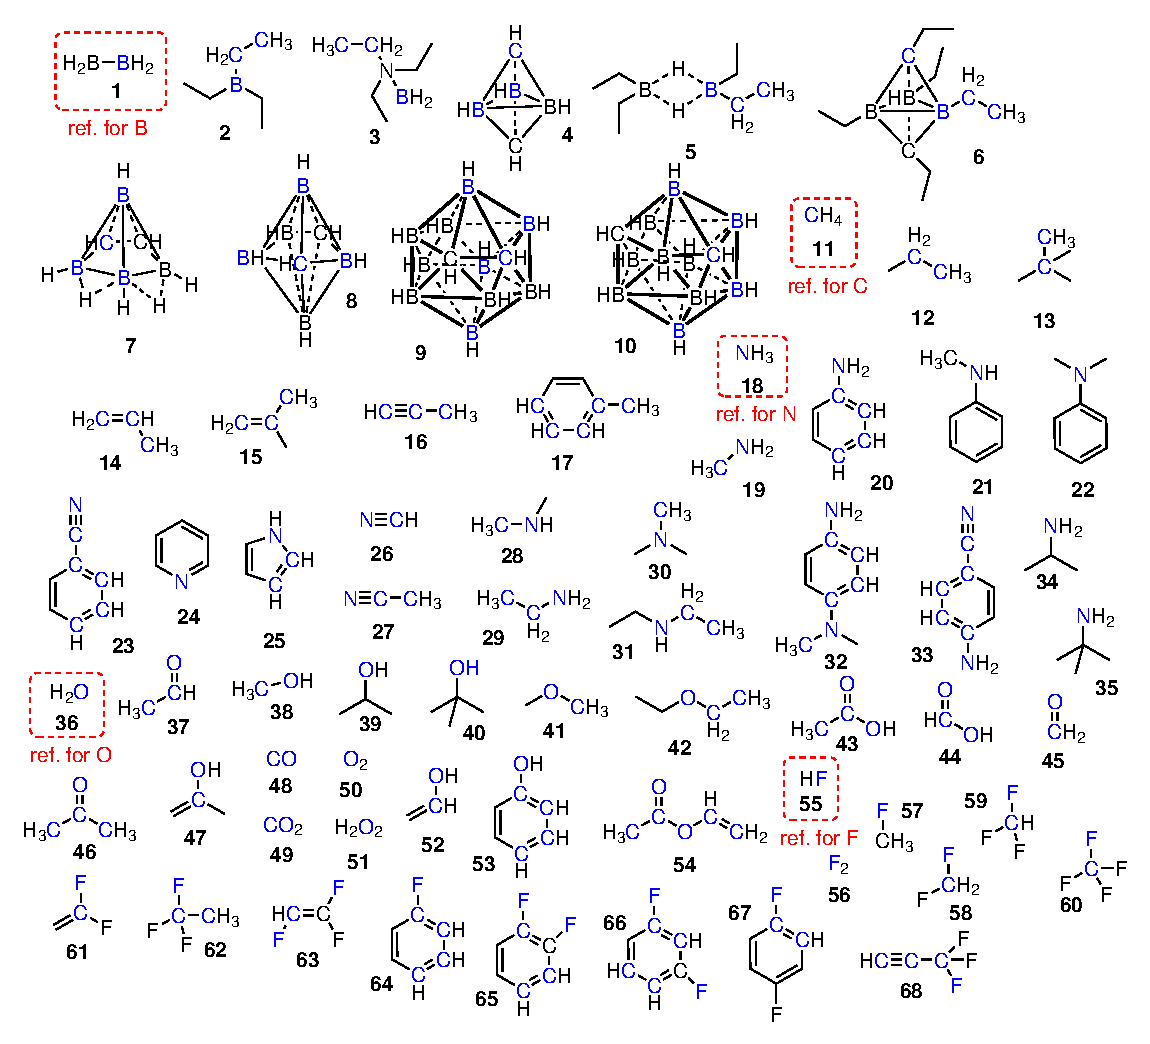
\includegraphics[width=\linewidth]{FigureS1}
	\caption{Molecules for the benchmark, from Ref.~\citenum{pueyobellafontPredictingCoreLevel2017}. The atoms for which experimental BE are provided are highlighted in blue.  The reference compounds used for each atom are highlighted in red.}
	\label{fig:core185}
\end{figure}


\begin{figure}[!h]
	\includegraphics[width=\linewidth]{FigureS2}
	\caption{Evolution of the surface energy (in \si{\joule\per\meter\squared}) for slabs of Ca, CaO, and \ce{CaH2} with increasing thickness ($N$) , as estimated by least-square fit of Eq.~(5) of the main text. For CaO, the surface energies of (110) and (111) are larger than \SI{1.25}{\joule\per\meter\squared}.}
	\label{fig:surf}
\end{figure}

\begin{table}[!h]
	\centering
	\caption{Comparison between experimental (from Ref.~\citenum{pueyobellafontPredictingCoreLevel2017}) and calculated (as computed with the \cpx[n]{0} protocol) absolute BE (in \si{\electronvolt}).}
	\label{tab:xpssjn}
	\begin{ruledtabular}
	\begin{tabular}{lcccc}
		
		& Reference & BE (exp.)  & BE(calc.)  & $\Delta$(calc. - exp.)\\
		\hline
		B 1s & \ce{H2B-BH2} & 196.50 & 201.47 & 4.97\\
		C 1s & \ce{CH4} & 290.90 & 297.04 & 6.14\\
		N 1s & \ce{NH3} & 405.60 & 413.58 & 7.98\\
		O 1s & \ce{H2O} & 539.70 & 548.79 & 9.09\\
		F 1s & \ce{HF} & 694.23 & 704.78 &10.55\\
		
	\end{tabular}
\end{ruledtabular}
\end{table}

\begin{figure}[!h]
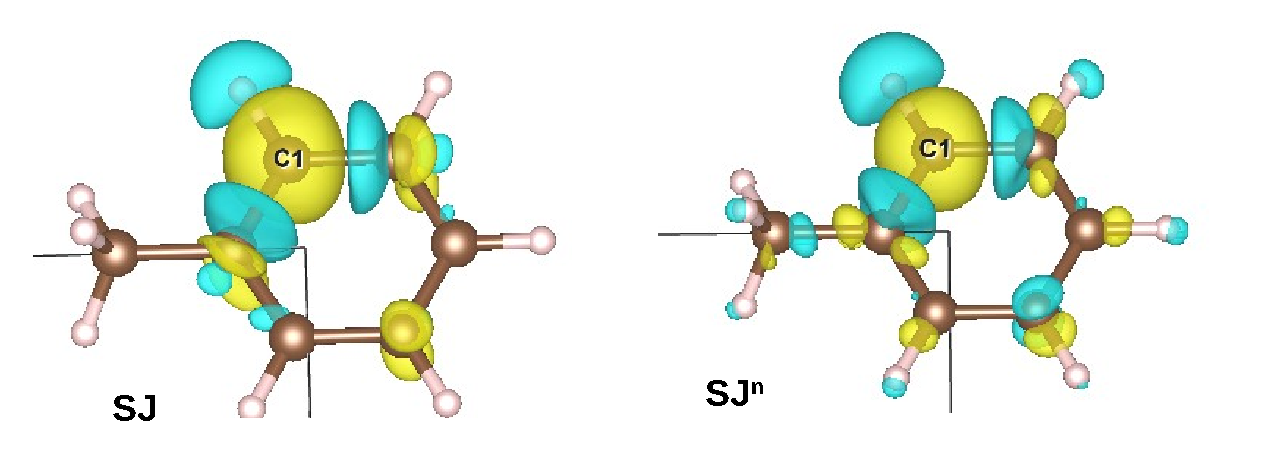
\includegraphics[width=\linewidth]{FigureS3}
\caption{Change in electron density (visualized with an isocontour of 0.003 a.u.) due to the creation of a core-hole in the 1s orbital of C1, with the SJ (left) or SJ\textsuperscript{n} (right) methods. Yellow (blue) corresponds to zone of depletion (increase) of the electron density.}
\end{figure}

\begin{figure}[!h]
\centering
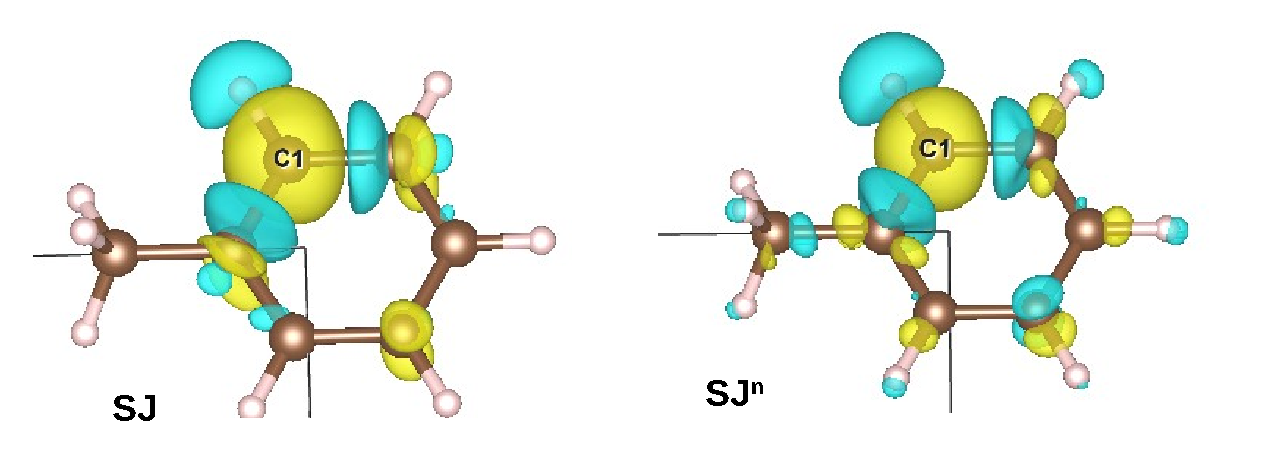
\includegraphics[width=\linewidth]{FigureS4}
\caption{Impact of the slab thickness (indicated as the number of layers, $N$) on the mean bulk (filled markers)  and surface (empty markers) \dbe{} (in \si{\electronvolt}), as computed with the SJ method and different reference energies. The vertical lines indicates standard deviation.}
\label{fig:slabsthicknessSJ}
\end{figure}

\begin{figure}[!h]
\centering
\includegraphics[width=\linewidth]{FigureS5}
\caption{Impact of the slab thickness (indicated as the number of layers) on the mean bulk (round markers)  and surface (square markers) \dbe{} (in \si{\electronvolt}), as computed with the SJ\textsuperscript{n} protocol and different references. The vertical lines indicates standard deviation.}
\label{fig:slabsthicknessSJn}
\end{figure}

\begin{table}
	\caption{Mean (and standard deviation) bulk and surface \dbe{} values  (in \si{\electronvolt}) for 6-layer (\ce{Ca^0}, CaO, and \ce{CaO.H2O}) and 12-layer (\ce{CaH2}) slabs, computed using the SJ method with various reference energies.}
	\begin{ruledtabular}
	\begin{tabular}{l cc c ccc}
		
		& \multicolumn{2}{c}{Ca 2s} &&  \multicolumn{3}{c}{O 1s}\\
		\cline{2-3} \cline{5-7}
		& Bulk & Surface & & Bulk & Surface & Hydroxyls\\
		\hline
		\multicolumn{7}{c}{SJ+$E_{ref}=0$}  \\
		\ce{Ca^0} &3.43 $\pm$ 0.04 & 3.90 $\pm$ 0.01 && --- & --- & ---\\
		\ce{CaH2} & 3.46 $\pm$ 0.02 & 3.45 $\pm$ 0.00 && --- & --- & ---\\
		CaO & 1.70 $\pm$ 0.02 & 2.33 $\pm$ 0.00 && -7.02 $\pm$ 0.02 & -7.54 $\pm$ 0.00 & ---\\
		\ce{CaO.H2O} & 1.25 $\pm$ 0.04 & 1.78 $\pm$ 0.00 && -7.50 $\pm$ 0.05 & -5.83 $\pm$ 0.00 & -5.90 $\pm$ 0.01\\
		\hline
		\multicolumn{7}{c}{SJ+$E_{ref}=E_F$}  \\
		\ce{Ca^0} &-0.36 $\pm$ 0.04 & 0.10 $\pm$ 0.01 && --- & --- & ---\\
		\ce{CaH2} & 0.39 $\pm$ 0.02 & 0.23 $\pm$ 0.00 && --- & --- & ---\\
		CaO & 0.04 $\pm$ 0.04 & 0.56 $\pm$ 0.00 && -2.99 $\pm$ 0.01 & -3.63 $\pm$ 0.00 & ---\\
		\ce{CaO.H2O} & 0.03 $\pm$ 0.06 & 0.59 $\pm$ 0.00 && -2.97 $\pm$ 0.05 & -1.33 $\pm$ 0.00 & -1.49 $\pm$ 0.00\\
		\hline
		\multicolumn{7}{c}{SJ+$E_{ref}=\varepsilon_{Ar,2s}$}  \\
		\ce{Ca^0} &1.05 $\pm$ 0.04 & 1.50 $\pm$ 0.00 && --- & --- & ---\\
		\ce{CaH2} & 0.51 $\pm$ 0.02 & 0.50 $\pm$ 0.00 && --- & --- & ---\\
		CaO & 0.24 $\pm$ 0.01 & 0.96 $\pm$ 0.00 && -3.55 $\pm$ 0.03 & -4.04 $\pm$ 0.00 & ---\\
		\ce{CaO.H2O} & 0.15 $\pm$ 0.05 & 0.63 $\pm$ 0.06 && -3.83 $\pm$ 0.08 & -1.63 $\pm$ 0.64 & -1.57 $\pm$ 0.70\\
		\hline
		\multicolumn{7}{c}{SJ+$E_{ref}=E_\infty$}  \\
		\ce{Ca^0} &1.04 $\pm$ 0.04 & 1.54 $\pm$ 0.01 && --- & --- & ---\\
		\ce{CaH2} & 0.54 $\pm$ 0.02 & 0.54 $\pm$ 0.00 && --- & --- & ---\\
		CaO & 0.29 $\pm$ 0.03 & 1.10 $\pm$ 0.00 && -3.53 $\pm$ 0.06 & -3.90 $\pm$ 0.00 & ---\\
		\ce{CaO.H2O} & 0.15 $\pm$ 0.05 & 0.69 $\pm$ 0.00 && -3.76 $\pm$ 0.04 & -2.03 $\pm$ 0.00 & -1.92 $\pm$ 0.00\\
		\hline
		\multicolumn{7}{c}{SJ+$E_{ref}=\phi$}  \\
		\ce{Ca^0} &4.83 $\pm$ 0.04 & 5.34 $\pm$ 0.01 && --- & --- & ---\\
		\ce{CaH2} & 3.61 $\pm$ 0.03 & 3.77 $\pm$ 0.00 && --- & --- & ---\\
		CaO & 1.96 $\pm$ 0.04 & 2.87 $\pm$ 0.00 && -7.55 $\pm$ 0.09 & -7.80 $\pm$ 0.00 & ---\\
		\ce{CaO.H2O} & 1.35 $\pm$ 0.03 & 1.88 $\pm$ 0.00 && -8.27 $\pm$ 0.05 & -6.53 $\pm$ 0.00 & -6.33 $\pm$ 0.00\\
		\end{tabular}
	\end{ruledtabular}
\end{table}

\begin{table}
	\caption{Mean (and standard deviation) bulk and surface \dbe{} values (in \si{\electronvolt}) for 6-layer (\ce{Ca^0}, CaO, and \ce{CaO.H2O}) and 12-layer (\ce{CaH2}) slabs, computed using the SJ\textsuperscript{n}  method with various reference energies.}
	\begin{ruledtabular}
	\begin{tabular}{l cc c ccc}
		& \multicolumn{2}{c}{Ca 2s} &&  \multicolumn{3}{c}{O 1s}\\
		\cline{2-3} \cline{5-7}
		& Bulk & Surface & & Bulk & Surface & Hydroxyls\\
		\hline
		\multicolumn{7}{c}{SJ$^n$+$E_{ref}=0$}  \\
		\ce{Ca^0} &1.58 $\pm$ 0.04 & 2.05 $\pm$ 0.01 && --- & --- & ---\\
		\ce{CaH2} & 2.06 $\pm$ 0.05 & 2.83 $\pm$ 0.00 && --- & --- & ---\\
		CaO & 0.82 $\pm$ 0.05 & 1.54 $\pm$ 0.00 && -8.90 $\pm$ 0.06 & -9.03 $\pm$ 0.00 & ---\\
		\ce{CaO.H2O} & 1.43 $\pm$ 0.05 & 2.64 $\pm$ 0.00 && -8.40 $\pm$ 0.04 & -6.38 $\pm$ 0.00 & -6.19 $\pm$ 0.00\\
		\hline
		\multicolumn{7}{c}{SJ$^n$+$E_{ref}=E_F$}  \\
		\ce{Ca^0} &-0.48 $\pm$ 0.03 & -0.02 $\pm$ 0.01 && --- & --- & ---\\
		\ce{CaH2} & -0.73 $\pm$ 0.03 & -0.29 $\pm$ 0.00 && --- & --- & ---\\
		CaO & -0.86 $\pm$ 0.05 & -0.01 $\pm$ 0.00 && -0.63 $\pm$ 0.14 & -0.79 $\pm$ 0.00 & ---\\
		\ce{CaO.H2O} & -0.56 $\pm$ 0.16 & 0.62 $\pm$ 0.00 && -0.43 $\pm$ 0.13 & 1.67 $\pm$ 0.00 & 1.96 $\pm$ 0.00\\
		\hline
		\multicolumn{7}{c}{SJ$^n$+$E_{ref}=\varepsilon_{Ar,2s}$}  \\
		\ce{Ca^0} &-1.57 $\pm$ 0.04 & -1.09 $\pm$ 0.00 && --- & --- & ---\\
		\ce{CaH2} & -2.07 $\pm$ 0.04 & -1.32 $\pm$ 0.01 && --- & --- & ---\\
		CaO & -1.12 $\pm$ 0.09 & -0.56 $\pm$ 0.00 && -4.66 $\pm$ 0.01 & -5.00 $\pm$ 0.00 & ---\\
		\ce{CaO.H2O} & 0.58 $\pm$ 0.04 & 1.43 $\pm$ 0.00 && -3.06 $\pm$ 0.09 & -1.42 $\pm$ 0.00 & -1.48 $\pm$ 0.01\\
		\hline
		\multicolumn{7}{c}{SJ$^n$+$E_{ref}=E_F'$}  \\
		\ce{Ca^0} &2.68 $\pm$ 0.04 & 3.14 $\pm$ 0.03 && --- & --- & ---\\
		\ce{CaH2} & 3.40 $\pm$ 0.04 & 3.87 $\pm$ 0.00 && --- & --- & ---\\
		CaO & 1.06 $\pm$ 0.10 & 2.08 $\pm$ 0.00 && -4.99 $\pm$ 0.19 & -4.93 $\pm$ 0.00 & ---\\
		\ce{CaO.H2O} & 0.31 $\pm$ 0.25 & 1.83 $\pm$ 0.00 && -5.84 $\pm$ 0.21 & -3.40 $\pm$ 0.00 & -2.88 $\pm$ 0.00\\
	\end{tabular}
\end{ruledtabular}
\end{table}



\begin{table}[!h]
	\caption{Experimental value of peak maximum energies  (in \si{\electronvolt}) for Ca, CaO, and  \ce{CaCO3}, from different sources. It is now recognized that for surfaces, a peak is not necessarily equivalent to a single binding energies (peak fitting is required), and that the spectra for pure CaO are difficult to obtain without contamination.\cite{dupinSystematicXPSStudies2000}}
	\begin{ruledtabular}
		\begin{tabular}{c ccc c ccc cl}
			\ce{Ca^0} & & \multicolumn{2}{c}{CaO} & & \multicolumn{3}{c}{\ce{CaCO3}} & Ref. & Note\\
			\cline{1-1} \cline{3-4} \cline{6-8}
			Ca 2s & & Ca 2s & O 1s  & & Ca 2s & O 1s & C 1s\\
			\hline
			438.8 & &---&---&& --- & --- &--- & \citenum{fuggleCorelevelBindingEnergies1980} & Relative to VBM\\
			436.6 & & 437.9 & 528.9& & 439.1 &531.6 & 289.7& \citenum{sosulnikovXrayPhotoelectronStudies1992}& Relative to C 1s = \SI{285.0}{\electronvolt}\\
			--- && 437.4 & 531.2&& 437.8 & 531.0 & 289.0 & \citenum{demriXPSStudyCalcium1995} & Relative to C 1s = \SI{284.6}{\electronvolt}\\
			$\sim$450 & & 441.0 & 532.2 & & --- & --- & --- & \citenum{ochsCO2ChemisorptionCa1998} & Relative to $E_F$ \\
			--- & & 439.0 & 531.9 & & 438.4 & 531.4 & 285.4 & \citenum{cristHandbookMonochromaticXPS2000a} & Relative to C 1s = \SI{285.0}{\electronvolt}\\
			442.5 & & 438.15 & 531.15 & & 439.08 & 531.58 & 290.08 & \citenum{cristXPSLibraryWebsite2021a} & Relative to C 1s = \SI{285.0}{\electronvolt}\\
			
		\end{tabular}
	\end{ruledtabular}
\end{table}

\begin{table}[!h]
\centering
\caption{Mean displacement (in \si{\angstrom}) of the calcium atoms of the slab due to the adsorption of a substrate.}
\label{tab:disp}
\begin{ruledtabular}
	\begin{tabular}{>{\bfseries}lcccc}
		& Ca & \ce{CaO} & \ce{CaO.H2O} & \ce{CaH2} \\
		\hline
		& \multicolumn{4}{c}{Hydrocarbons} \\
		a & 0.045 & 0.085 & 0.008 & 0.011 \\
		b & 0.047 & 0.013 & 0.007 & 0.014 \\
		c & 0.052 & 0.014 & 0.007 & 0.011 \\
		d & 0.051 & 0.035 & 0.007 & 0.020 \\
		\hline
		& \multicolumn{4}{c}{Polar molecules} \\
		e & 0.086 & 0.009 & 0.009 & 0.037 \\
		f & 0.055 & 0.010 & 0.010 & 0.067 \\
		g & 0.065 & 0.013 & 0.012 & 0.015 \\
		h & 0.051 & 0.027 & 0.008 & 0.013 \\
		\hline
		& \multicolumn{4}{c}{Protic molecules} \\
	i & 0.054 & 0.077 & 0.029 & 0.019 \\
	j & 0.067 & 0.091 & 0.044 & 0.057 \\
	\end{tabular}
\end{ruledtabular}
\end{table}

\newcommand{\XPSsa}[2]{
	\begin{figure}[!h]
		\centering
		\includegraphics[width=\linewidth]{Figure#1}
		\caption{Difference (dotted line) between the XPS spectra before (dashed line) and after (solid line) adsorption for compounds \textbf{#2} on various substrates, as computed using the \cpx{E_\infty} protocol. Letters indicate mean binding energies for bulk (``b"), surface (``s", with $\star$ marking the atom closest to the adsorbate), surface hydroxides (``h"), and different atoms of the adsorbate.}
		\label{fig:spectraXPSads#2}
	\end{figure}
}

\newcommand{\XPSsab}[4]{
	\begin{figure}[p]
		\centering
		\includegraphics[width=\linewidth]{Figure#1}
		\includegraphics[width=\linewidth]{Figure#2}
		\caption{Difference (dotted line) between the XPS spectra before (dashed line) and after (solid line) adsorption for compounds (a) \textbf{#3} and (b) \textbf{#4} on various substrates, as computed using the \cpx{E_\infty} protocol. Letters indicate mean binding energies for bulk (``b"), surface (``s", with $\star$ marking the atom closest to the adsorbate), surface hydroxides (``h"), and different atoms of the adsorbate.}
		\label{fig:spectraXPSads#3#4}
	\end{figure}
}

\XPSsab{S6a}{S6b}{b}{d}
\XPSsab{S7a}{S7b}{f}{g}
\XPSsa{S8}{i}

\clearpage
\bibliography{biblio}
	
\end{document}